\section{What is Maching Learning}
\noindent
{\color{LightRubineRed} \rule{\linewidth}{1mm} }
让机器去学习。有时候规则很难定义,比如怎么定义什么是一颗树。而让机器通过数据学习就会使问题变简单了。可以让机器自动挖掘一些模式。\par
\subsection{Machine learning}
improving some Performance measure with experience computed from Data. \par
use \textcolor{Mycolor1}{data} to compute hypothesis g that \textcolor{Mycolor1}{approximates} target f. \par

\begin{center}
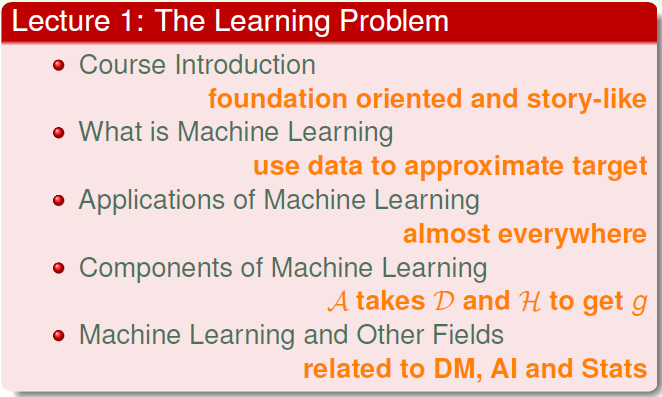
\includegraphics[width=10cm, height=6cm]{lecture1_sum}\\
\end{center}

\noindent
{\color{RubineRed} \rule{\linewidth}{1mm} }
% {\color{LightRubineRed} \rule{\linewidth}{1mm} }
